
\date{\today}
\title{Local Network Analysis}


\documentclass[12pt]{article}

\usepackage{graphicx}

\author{
  Singhal, Madhur\\
  \texttt{2015CS10235}
  \and
  Chhajwani, Anant\\
  \texttt{2015CS50281}
}

\begin{document}
\maketitle


\section{Introduction}
Nmap is a free and open source utility for network exploration and security auditing. It is primarily used for probing networks to reveal the active hosts and discover the ports and services that the hosts respond to. 
\paragraph{}
In this assignment we created a script to monitor a local subnet and track the number of hosts up at different points in time. We also ran nmap by itself on the local subnet to identify different hosts and services running.

\section{Number of Hosts}
The number of hosts was found to vary between 0 and 35. At nights, because of the LAN ban the number of hosts decreased significantly. Some hosts which are still up could be routers or mis-configured hosts. A graph is provided which plots the time dependence of the number of hosts. The median number of hosts is 17.

\paragraph{}
\begin{center}
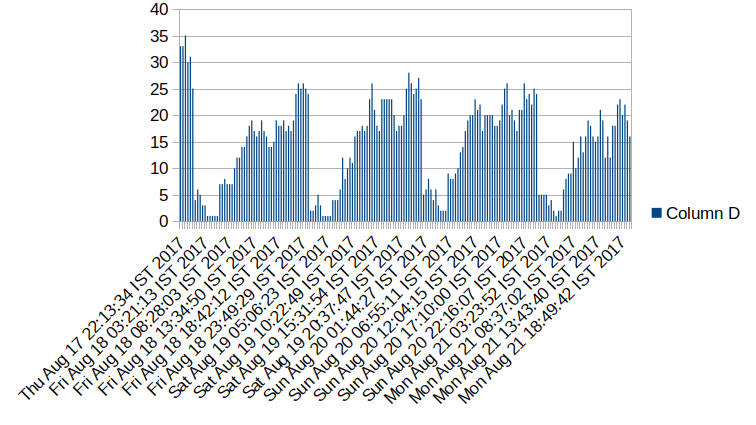
\includegraphics[scale=1.0]{gr.png}
\end{center}


\section{Hosts and Services}

This question seems a bit broad, nevertheless I have provided a list of 16 hosts up when I checked today and their services.

\begin{enumerate}


\item Nmap scan report for 10.203.148.1
\begin{itemize}


\item Host is up (0.031s latency).
\item Not shown: 996 closed ports
\item PORT    STATE SERVICE
\item 22/tcp  open  ssh
\item 23/tcp  open  telnet
\item 80/tcp  open  http
\item 443/tcp open  https

\end{itemize}

\item Nmap scan report for 10.203.148.15
\begin{itemize}
\item Host is up (0.064s latency).
\item Not shown: 994 closed ports
\item PORT      STATE    SERVICE
\item 668/tcp   filtered mecomm
\item 1079/tcp  filtered asprovatalk
\item 3851/tcp  filtered spectraport
\item 5906/tcp  filtered unknown
\item 7443/tcp  filtered oracleas-https
\item 49175/tcp filtered unknown
\end{itemize}

\item Nmap scan report for 10.203.148.32
\begin{itemize}
\item Host is up (0.073s latency).
\item Not shown: 986 closed ports
\item PORT      STATE    SERVICE
\item 135/tcp   open     msrpc
\item 139/tcp   open     netbios-ssn
\item 445/tcp   open     microsoft-ds
\item 1935/tcp  open     rtmp
\item 2869/tcp  open     icslap
\item 3517/tcp  filtered 802-11-iapp
\item 5357/tcp  open     wsdapi \item 
8080/tcp  open     http-proxy\item 
10025/tcp filtered unknown\item 

49152/tcp open     unknown\item 
49153/tcp open     unknown\item 
49154/tcp open     unknown\item 
49155/tcp open     unknown\item 
49156/tcp open     unknown
\end{itemize}

\item Nmap scan report for 10.203.148.72
\begin{itemize}\item 
Host is up (0.013s latency).\item 
Not shown: 979 closed ports\item 
PORT      STATE    SERVICE\item 
80/tcp    open     http\item 
135/tcp   open     msrpc\item 
139/tcp   open     netbios-ssn\item 
301/tcp   filtered unknown\item 
443/tcp   open     https\item 
445/tcp   open     microsoft-ds\item 
1718/tcp  filtered h323gatedisc\item 
2909/tcp  filtered funk-dialout\item 
5033/tcp  filtered jtnetd-server\item 
5357/tcp  open     wsdapi\item 
5925/tcp  filtered unknown\item 
8200/tcp  filtered trivnet1\item 
9011/tcp  filtered unknown\item 
30718/tcp filtered unknown\item 
49152/tcp open     unknown\item 
49153/tcp open     unknown\item 
49154/tcp open     unknown\item 
49155/tcp open     unknown\item 
49156/tcp open     unknown\item 
49157/tcp open     unknown\item 
49999/tcp filtered unknown
\end{itemize}

\item Nmap scan report for 10.203.148.82
\begin{itemize}\item 
Host is up (0.013s latency).\item 
All 1000 scanned ports on 10.203.148.82 are filtered
\end{itemize}

\item Nmap scan report for 10.203.148.94
\begin{itemize}\item 
Host is up (0.15s latency).\item 
Not shown: 986 closed ports\item 
PORT      STATE    SERVICE\item 
714/tcp   filtered iris-xpcs\item 
1022/tcp  filtered exp2\item 
1028/tcp  filtered unknown\item 
1049/tcp  filtered td-postman\item 
1102/tcp  filtered adobeserver-1\item 
1352/tcp  filtered lotusnotes\item 
1687/tcp  filtered nsjtp-ctrl\item 
2008/tcp  filtered conf\item 
2323/tcp  filtered 3d-nfsd\item 
2525/tcp  filtered ms-v-worlds\item 
3880/tcp  filtered igrs\item 
5051/tcp  filtered ida-agent\item 
5910/tcp  filtered cm\item 
44442/tcp filtered coldfusion-auth
\end{itemize}

\item Nmap scan report for 10.203.148.125
\begin{itemize}\item 
Host is up (0.035s latency).\item 
Not shown: 999 closed ports\item 
PORT   STATE SERVICE\item 
22/tcp open  ssh
\end{itemize}

\item Nmap scan report for 10.203.148.144
\begin{itemize}\item 
Host is up (0.034s latency).\item 
Not shown: 995 closed ports\item 
PORT     STATE    SERVICE\item 
106/tcp  filtered pop3pw\item 
1352/tcp filtered lotusnotes\item 
1900/tcp filtered upnp\item 
2608/tcp filtered wag-service\item 
8652/tcp filtered unknown
\end{itemize}

\item Nmap scan report for 10.203.148.162
\begin{itemize}\item 
Host is up (0.029s latency).\item 
Not shown: 986 closed ports\item 
PORT      STATE    SERVICE\item 
42/tcp    filtered nameserver\item 
135/tcp   open     msrpc\item 
139/tcp   open     netbios-ssn\item 
264/tcp   filtered bgmp\item 
306/tcp   filtered unknown
\end{itemize}

\item Nmap scan report for 10.203.149.14
\begin{itemize}\item 
Host is up (0.029s latency).\item 
All 1000 scanned ports on 10.203.149.14 are closed
\end{itemize}

\item Nmap scan report for 10.203.149.20
\begin{itemize}\item 
Host is up (0.033s latency).\item 
Not shown: 999 closed ports\item 
PORT   STATE    SERVICE\item 
21/tcp filtered ftp
\end{itemize}

\item Nmap scan report for 10.203.149.30
\begin{itemize}\item 
Host is up (0.022s latency).\item 
Not shown: 999 filtered ports\item 
PORT     STATE SERVICE\item 
6646/tcp open  unknown
\end{itemize}

\item Nmap scan report for 10.203.149.59
\begin{itemize}\item 
Host is up (0.025s latency).\item 
All 1000 scanned ports on 10.203.149.59 are closed
\end{itemize}

\item Nmap scan report for 10.203.149.62
\begin{itemize}\item 
Host is up (0.056s latency).\item 
Not shown: 979 closed ports\item 
PORT      STATE    SERVICE\item 
135/tcp   open     msrpc\item 
139/tcp   open     netbios-ssn\item 
445/tcp   open     microsoft-ds\item 
554/tcp   open     rtsp\item 
555/tcp   filtered dsf\item 
1148/tcp  filtered elfiq-repl\item 
1500/tcp  filtered vlsi-lm\item 
1935/tcp  open     rtmp\item 
2869/tcp  open     icslap\item 
5357/tcp  open     wsdapi\item 
5862/tcp  filtered unknown\item 
8089/tcp  filtered unknown\item 
10243/tcp open     unknown\item 
49152/tcp open     unknown\item 
49153/tcp open     unknown\item 
49154/tcp open     unknown\item 
49155/tcp open     unknown\item 
49156/tcp open     unknown\item 
49158/tcp open     unknown\item 
49165/tcp open     unknown
\end{itemize}

\item Nmap scan report for 10.203.149.115
\begin{itemize}\item 
Host is up (0.078s latency).\item 
Not shown: 993 filtered ports\item 
PORT     STATE SERVICE\item 
80/tcp   open  http\item 
515/tcp  open  printer\item 
1801/tcp open  msmq\item 
2103/tcp open  zephyr-clt\item 
2105/tcp open  eklogin\item 
2107/tcp open  msmq-mgmt\item 
2869/tcp open  icslap
\end{itemize}

 \item Nmap scan report for 10.203.149.155
 \begin{itemize}\item 
Host is up (0.042s latency).\item 
Not shown: 999 filtered ports\item 
PORT   STATE SERVICE\item 
80/tcp open  http
\end{itemize}

\end{enumerate}


\section{Gateways and DNS Servers}

The DNS Servers \textbf{10.10.1.2 and 10.10.2.2}, are used in IIT Delhi for serving DNS requests of users. Many users also use external DNS servers like Google's 8.8.8.8 for their DNS needs.\\

The gateways are different for each area and I didn't find any list of them all. For my hostel (Jwalamukhi) the LAN gateways seem to be \textbf{10.254.203.6 and 10.254.203.2}. \\

For Vision Lab in Bharti Building, the gateways are \textbf{10.254.208.2 and 10.254.208.6}.




\end{document}